\documentclass[aspectratio=169]{beamer}
\usetheme{Singapore}
\setbeamertemplate{caption}[numbered]
\addtobeamertemplate{navigation symbols}{}{%
    \usebeamerfont{footline}%
    \usebeamercolor[fg]{footline}%
    \hspace{1em}%
    \raisebox{1.4pt}[0pt][0pt]{\insertframenumber/\inserttotalframenumber}
}

\usefonttheme[onlymath]{serif}

\usepackage{cmap}
\usepackage[english]{babel}
\usepackage[T1]{fontenc}
\usepackage[utf8]{inputenc}
\usepackage[kerning=true]{microtype}
\usepackage{lmodern}

\usepackage{amsmath}
\usepackage{amsfonts}
\usepackage{amssymb}
\usepackage{amsthm}

\usepackage{mathtools}
\usepackage{wrapfig}
\usepackage{enumitem}
\usepackage{tikz}
\usepackage{xcolor}
\usetikzlibrary{positioning}

\usepackage[
    backend=biber,
    style=numeric,
]{biblatex}
\usepackage{graphicx}
\usepackage[justification=centering]{caption}
\usepackage{csquotes}

\graphicspath{{../images/}}

\addbibresource{../report/report.bib}
\renewcommand*{\bibfont}{\footnotesize}

\AtBeginSection[]
{
  \begin{frame}
    \frametitle{Plan}
    \tableofcontents[currentsection]
  \end{frame}
}


\theoremstyle{definition}
\newtheorem*{exemple}{Example}

\renewcommand{\leq}{\leqslant}
\renewcommand{\geq}{\geqslant}


\title{\textbf{Image Colorization using DCGANs}}

\author{
    \texorpdfstring{%
    \begin{columns}
        \column{.5\linewidth}
        \centering
        \textbf{Nathan Frison} \\ \texttt{nathan.frison@ens.psl.eu}
        \column{.5\linewidth}
        \centering
        \textbf{Antoine Groudiev} \\ \texttt{antoine.groudiev@ens.psl.eu}
    \end{columns}
    }
    {Antoine Groudiev, Silviu Maniu}
}

\titlegraphic{
\includegraphics[height=1.6cm]{logo-ens-psl.png}}

\date{\today}

\begin{document}
\frame{\titlepage}

\begin{frame}{Image colorization}
    \begin{figure}
        \centering
        \begin{tikzpicture}
            \node at (0,0) {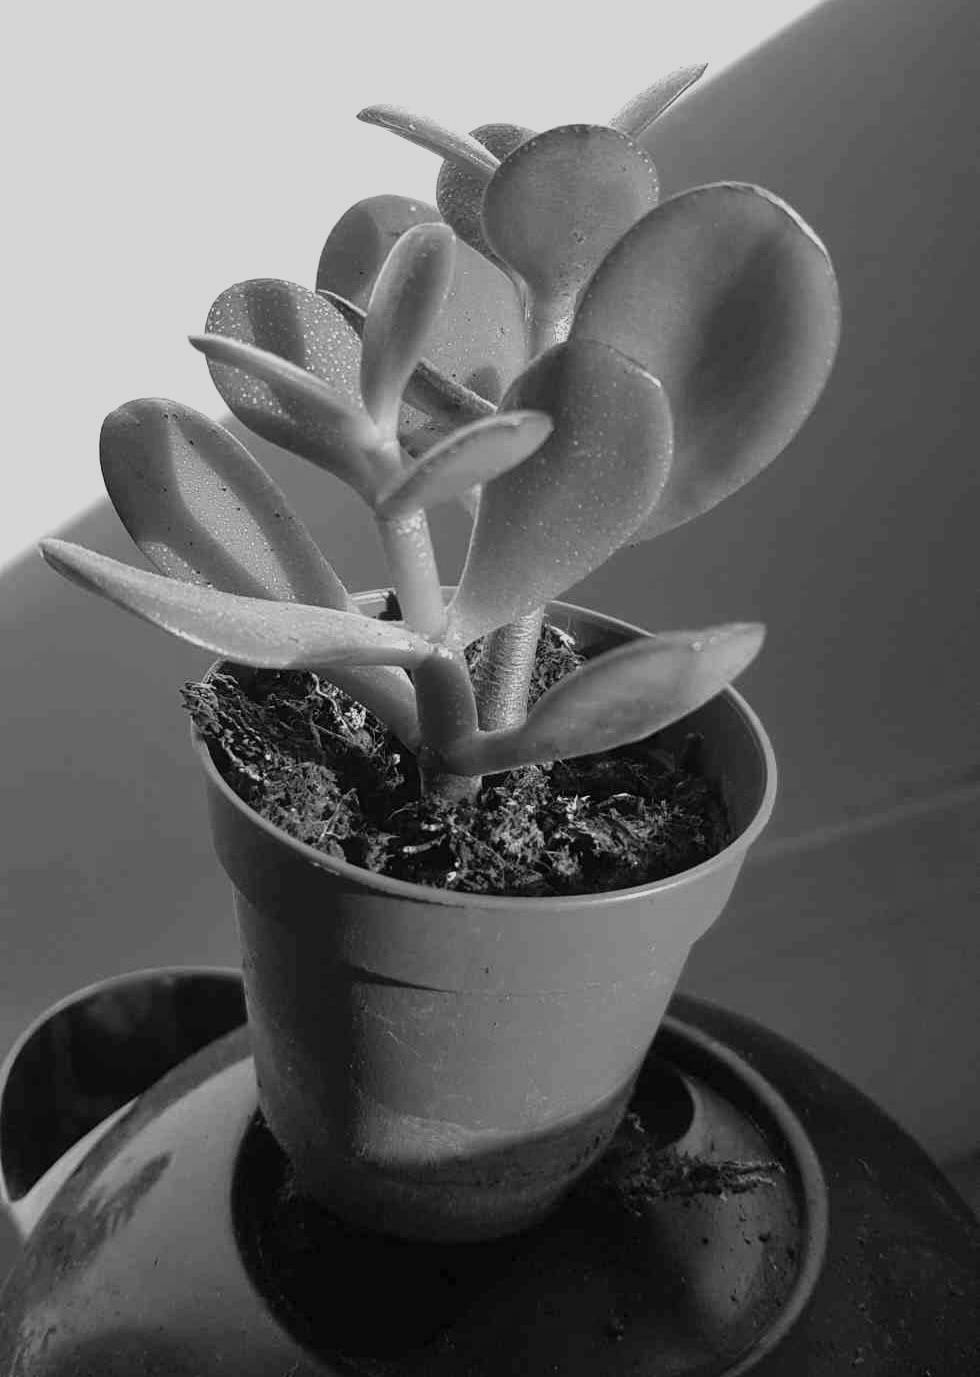
\includegraphics[width=.25\textwidth]{gray-plante.jpg}};
            \node at (0,-2.8) {Grayscale image};

            \draw[->, very thick] (2,-.2) -- ++(1,0);
            \draw[draw=black, thick, fill=orange!60, rounded corners] (3.2,-1.5) rectangle ++(3.5,2.5) node[pos=.5] {Neural network};
            \draw[->, very thick] (7,-.2) -- ++(1,0);

            \node at (10,0) {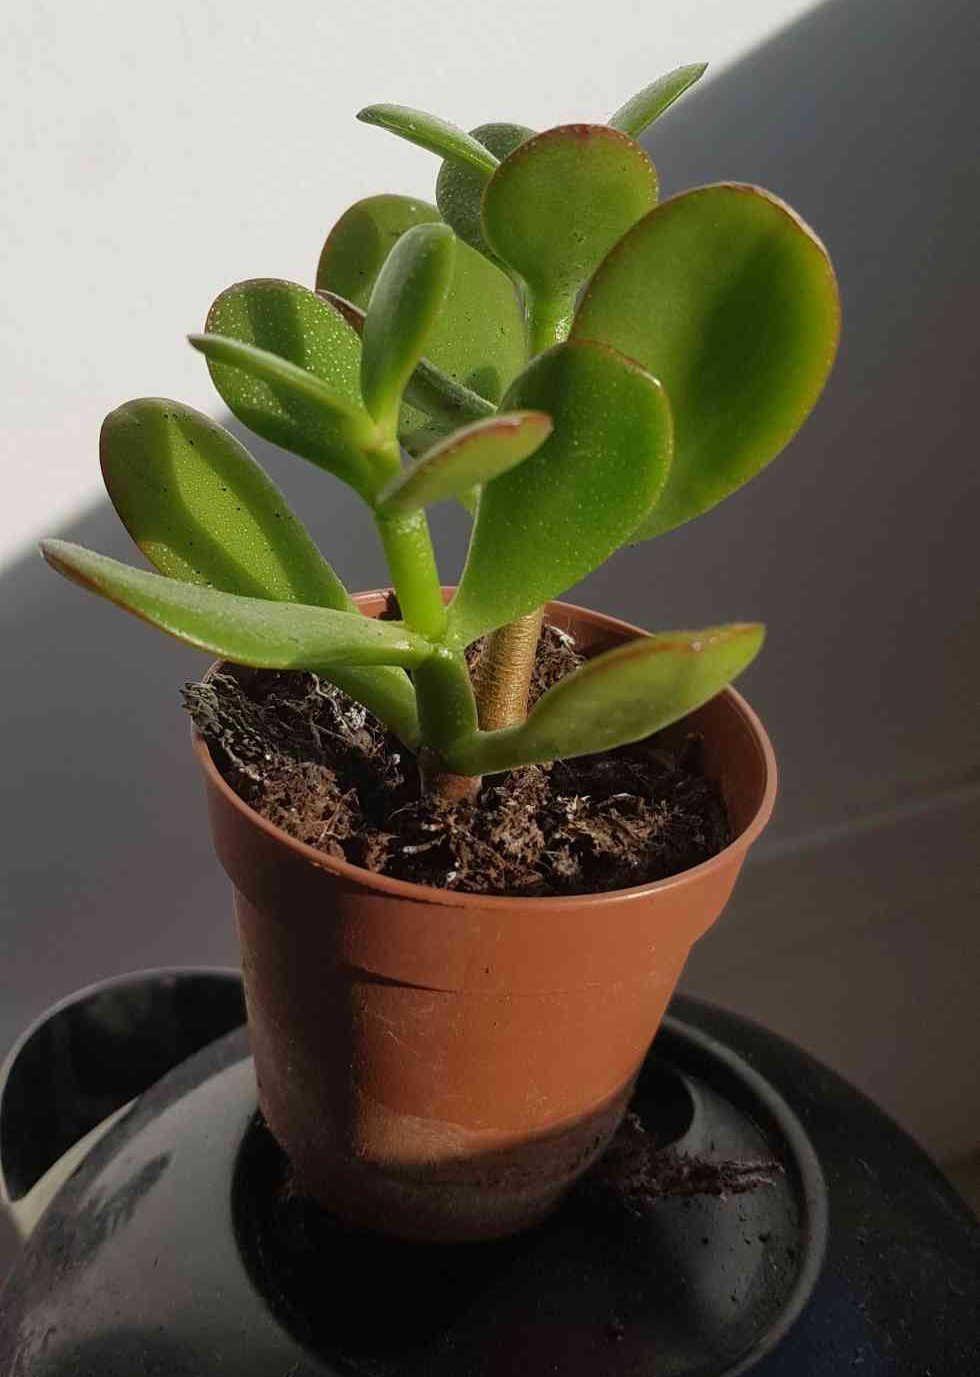
\includegraphics[width=.25\textwidth]{plante.jpg}};
            \node at (10,-2.8) {Colorized image};
        \end{tikzpicture}
    \end{figure}
\end{frame}

\begin{frame}{Generative Adversarial Networks (GANs)}
    \begin{figure}
    \centering
    \begin{tikzpicture}[scale=.9]
        \draw[draw=black, thick, fill=gray!40, rounded corners] (0, -1) rectangle ++(1.3, 2.7) node[pos=.5] {$\begin{bmatrix}z_0\\z_1\\\dots\\z_n\end{bmatrix}$};
        \node at (0.8,-1.4) {Sample from $p_z$};

        \draw[->, very thick] (1.4,0.3) -- ++(1,0);
        \draw[draw=black, thick, fill=orange!60, rounded corners] (2.5, -.7) rectangle ++(3, 2) node[pos=.5] {Generator};
        \draw[->, very thick] (5.7,0.3) -- ++(.7,0);

        \node at (7.6,0.3) {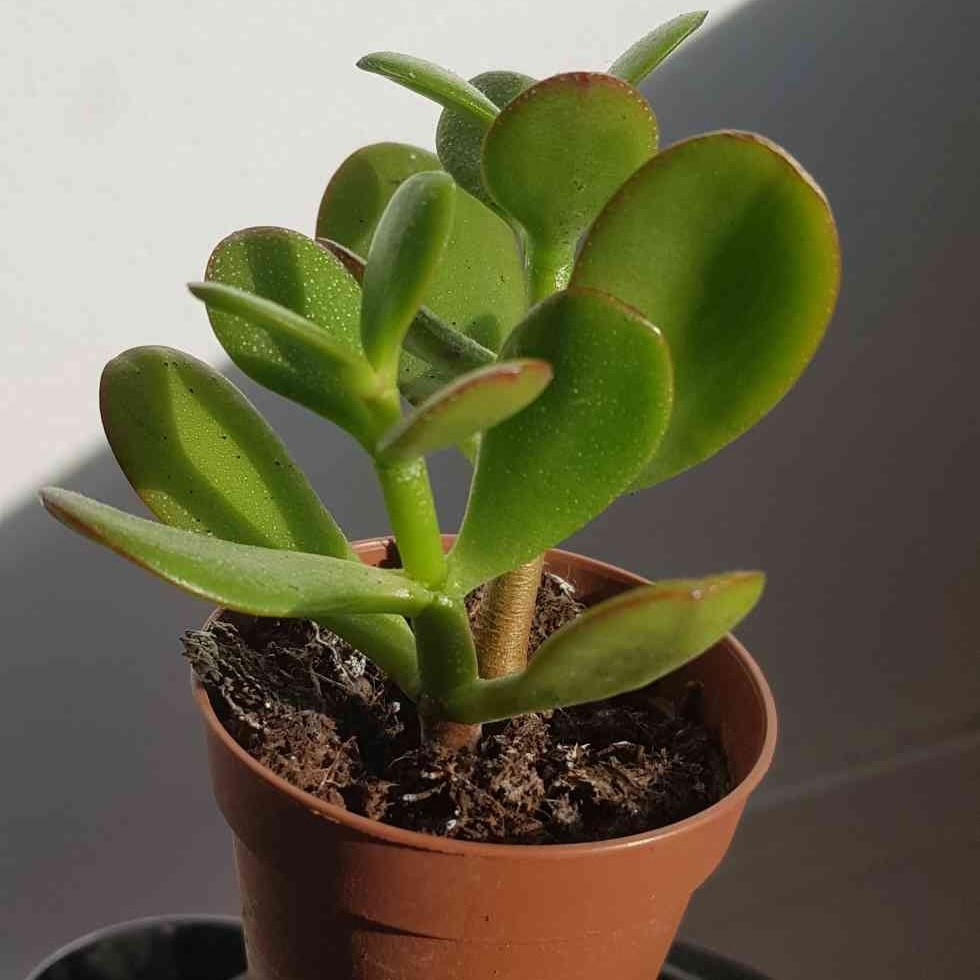
\includegraphics[width=1.8cm]{plante-sq.jpg}};
        \node at (7.6,1.6){Generated image};
        \node at (7.6,-2.5) {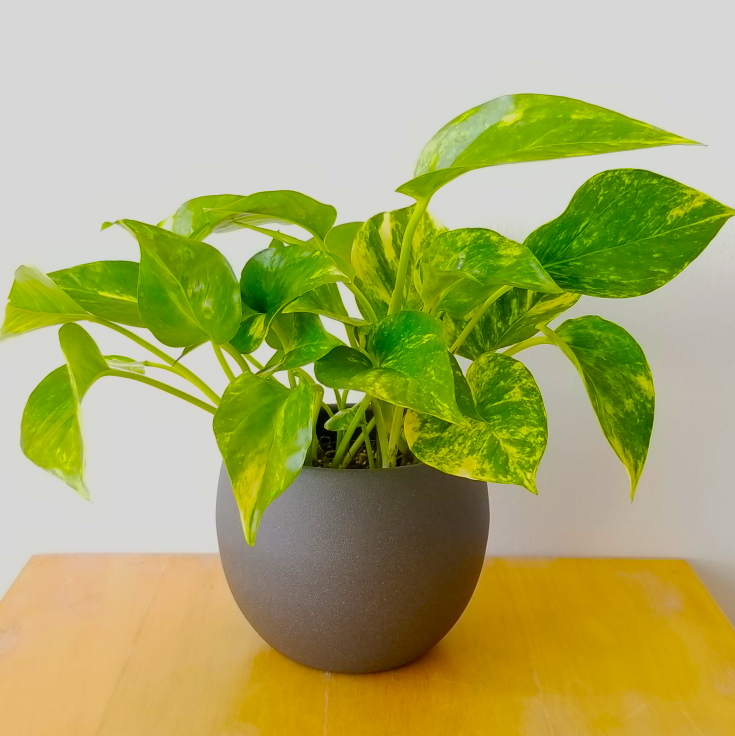
\includegraphics[width=1.8cm]{plante2.png}};
        \node at (7.6,-3.8){Dataset image};

        \draw[->, very thick] (8.7,0.3) -- ++(1,0);
        \draw[->, very thick] (8.7,-3.3) -- ++(.6,0) -- ++(0, 3.2) -- ++(.4, 0);
        
        \draw[draw=black, thick, fill=cyan!60, rounded corners] (10, -.7) rectangle ++(3, 2) node[pos=.5] {Discriminator};

        \draw[->, very thick] (13.1,.3) -- ++(.6,0) node[right] {$[0,1]$};
    \end{tikzpicture}
    \end{figure}
\end{frame}

\begin{frame}{References}
    
\end{frame}

\end{document}